\begin{code}[hide]
module slides.Tsinghua-PL-seminar.sections.newrcch where

open import Data.Nat using (ℕ)
open import Data.Product using (_×_ ; proj₁ ; proj₂)
open import Word.Base using (Word ; WRel ; ε ; _•_)
open import Notations using (₁₊ ; ₂₊ ; ₃₊ ; ₄₊)

infix 4 _SRel,_===_ _~_ _≐_ _VRel,_===_
infixl 10 _↑ _↓
infixr 8 _^_
infixr 7 _·_

postulate
  Gen : ℕ → Set
  Bits : ℕ → Set
  𝔽 : Set
  _^_ : ∀ {n} → Word (Gen n) → ℕ → Word (Gen n)
  _↑ _↓ : ∀ {n} → Word (Gen n) → Word (Gen n)
  H Z CZ CH °CZ °CH CZ₂₀ CH₂₀ PP : ∀ {n} → Word (Gen n)
  Λ□ : ℕ → ∀ {n} → Word (Gen n)
  √2^_ : ℕ → 𝔽
  _·_ : 𝔽 → ∀ {n} → (Bits n → Bits n → 𝔽) → (Bits n → Bits n → 𝔽)
  _≐_ : ∀ {n} → (Bits n → Bits n → 𝔽) → (Bits n → Bits n → 𝔽) → Set
  _VRel,_===_ : (n : ℕ) → WRel (Gen n)
  proof-elided : ∀ {A : Set} → A

Circuit : ℕ → Set
Circuit n = Word (Gen n)

private variable
  n : ℕ
\end{code}
%% Part 6d — Real-Clifford+CH (branch v-office-Cli-CH).

\begin{frame}{Real-Clifford+$CH$: Clément's complete equational theory \New}
\begin{columns}[c]
\begin{column}{0.53\textwidth}
\renewcommand{\AgdaCodeStyle}{\scriptsize}
\small A.\ Clément, arXiv:2602.06644: a 13-page paper, \alert{264 pages} of appendix.
\begin{code}
data Gate : ℕ → Set where
  H-gate  : Gate 1
  Z-gate  : Gate 1
  CZ-gate : Gate 2
  CH-gate : Gate 2

Ex : Circuit (₂₊ n)   -- Equation (8): the swap is a definition
Ex = CZ • H ↓ • H ↑ • CZ • H ↓ • H ↑ • CZ • H ↓ • H ↑
\end{code}
\begin{code}[hide]
\end{code}
\vspace{-6pt}
{\scriptsize 23 rules: (1)--(19) of Figure 4 minus (8), and the 5 swap rules of Remark 1;
a sample:}
\begin{code}
data _SRel,_===_ : (n : ℕ) → WRel (Gen n) where
  order-HZ : (₁₊ n) SRel, (H • Z) ^ 8 === ε
  merge-CZ    : (₂₊ n) SRel, CZ • °CZ === Z ↓
  slide-CH    : (₂₊ n) SRel, CH • H ↑ • Z ↑ • CH • H ↑
                             === H ↑ • Z ↑ • CH • H ↑ • CH
  square-CCZX   : (₃₊ n) SRel, (CH ↓ • CZ₂₀) ^ 4 === CZ ↑
  conj-PP       : (₃₊ n) SRel, CZ ↑ • PP ↓ === PP ↓ • CH ↑
  box-Z : ∀ k → (₁₊ (₄₊ k)) SRel, Z ↓ • Λ□ (₄₊ k) === Λ□ (₄₊ k) • Z ↓
\end{code}
\end{column}
\begin{column}{0.44\textwidth}
\centering
{\small the swap, by definition (8):}\\[2pt]
\begin{quantikz}[row sep=0.25cm,column sep=0.14cm,font=\scriptsize]
 & \swap{1} & \\
 & \targX{} &
\end{quantikz}
$=$
\begin{quantikz}[row sep=0.25cm,column sep=0.14cm,font=\scriptsize]
 & \ctrl{1} & \gate{H} & \ctrl{1} & \gate{H} & \ctrl{1} & \gate{H} & \\
 & \control{} & \gate{H} & \control{} & \gate{H} & \control{} & \gate{H} &
\end{quantikz}

\vspace{8pt}
{\small rule (11) \aid{slide-CH}:}\\[2pt]
\begin{quantikz}[row sep=0.25cm,column sep=0.12cm,font=\scriptsize]
 & \ctrl{1} & \gate{H} & \gate{Z} & \ctrl{1} & \gate{H} & \\
 & \gate{H} & & & \gate{H} & &
\end{quantikz}
$=$
\begin{quantikz}[row sep=0.25cm,column sep=0.12cm,font=\scriptsize]
 & \gate{H} & \gate{Z} & \ctrl{1} & \gate{H} & \ctrl{1} & \\
 & & & \gate{H} & & \gate{H} &
\end{quantikz}

\vspace{6pt}
{\scriptsize wire 0 is the bottom wire; $CH$ is controlled by wire 1.\\
(19) is a \alert{schema}: one rule per width $\ge5$, about the multi-controlled
box $\Lambda\square$ of Definition 2.4, defined by recursion.}
\end{column}
\end{columns}
\end{frame}

\begin{frame}{A matrix semantics over $\mathbb{Z}[\sqrt2]$ \New}
\begin{columns}[c]
\begin{column}{0.52\textwidth}
\renewcommand{\AgdaCodeStyle}{\scriptsize}
\small Gate matrices are taken $\times\sqrt2$, so entries lie in
$\mathbb{Z}[\sqrt2]$; the power of $\frac1{\sqrt2}$ is kept apart:
\begin{code}
Op : ℕ → Set
Op n = Bits n → Bits n → 𝔽

Scaled : ℕ → Set
Scaled n = ℕ × Op n          -- (ℓ , M)  reads  (1/√2)^ℓ · M

_~_ : Scaled n → Scaled n → Set
s ~ t = ((√2^ proj₁ t) · proj₂ s) ≐ ((√2^ proj₁ s) · proj₂ t)
\end{code}
\begin{code}[hide]
postulate ⟦_⟧ : ∀ {n} → Circuit n → Scaled n
\end{code}
\begin{itemize}
  \item matrices are computed on stored \alert{tries} \aid{Mat k};
  \item \textbf{soundness} (Prop.\ 3.1): each relator checked \emph{once}, by
        \aid{refl} on tries at the width it is drawn on; \aid{localise} /
        \aid{by-relator} lift it to \emph{every} width;
  \item the schema (19) at every width by a symbolic lemma: the box is
        $(\frac1{\sqrt2})^\ell$ times a diagonal sign.
\end{itemize}
\end{column}
\begin{column}{0.45\textwidth}
\centering
\begin{tikzpicture}[x=5.5mm,y=5.5mm,font=\scriptsize]
  \node at (-1.6,2) {$\tfrac{1}{\sqrt2}\;\cdot$};
  \draw[thick] (-0.3,-0.2) -- (-0.4,-0.2) -- (-0.4,4.2) -- (-0.3,4.2);
  \draw[thick] (4.3,-0.2) -- (4.4,-0.2) -- (4.4,4.2) -- (4.3,4.2);
  \foreach \r/\row in {0/{1,1,0,0},1/{1,-1,0,0},2/{0,0,1,1},3/{0,0,1,-1}} {
    \foreach \e [count=\c] in \row {
      \node at (\c-0.5,3.5-\r) {$\e$};
    }
  }
  \node[font=\scriptsize,align=center] at (2,-1) {$I\otimes H$ as $(1,M)$, $M$ over $\mathbb{Z}[\sqrt2]$};
\end{tikzpicture}

\vspace{8pt}
\begin{code}
axiom-sound : {w v : Circuit n} →
              n VRel, w === v → ⟦ w ⟧ ~ ⟦ v ⟧
\end{code}
\begin{code}[hide]
axiom-sound = proof-elided
\end{code}
{\scriptsize \texttt{Real-Clifford+CH/Semantics/Scaled.agda}, \texttt{Soundness.agda}}
\end{column}
\end{columns}
\end{frame}

\begin{frame}{Completeness: the paper's back-and-forth argument \New}
\begin{columns}[c]
\begin{column}{0.53\textwidth}
\centering
\begin{tikzpicture}[>={Stealth[length=1.8mm]}]
  \node[draw=newC,fill=softnew,rounded corners=2pt,font=\scriptsize,align=center,minimum height=10mm,text width=24mm] (C) at (0,0) {$n$-qubit circuits\\Figure 4};
  \node[draw=accent,fill=soft,rounded corners=2pt,font=\scriptsize,align=center,minimum height=10mm,text width=24mm] (P) at (4,0) {words over $P$\\Figure 8 (27 rules)};
  \node[draw=paperC,fill=softpaper,rounded corners=2pt,font=\scriptsize,align=center,minimum height=10mm,text width=24mm] (O) at (4,-2.6) {$O_{2^n}(\mathbb{Z}[\frac1{\sqrt2}])$\\Figure 7 (13 rules)};
  \draw[->,thick] (C.10) -- node[above,font=\scriptsize]{encode $e$} (P.170);
  \draw[->,thick] (P.190) -- node[below,font=\scriptsize]{decode $d$} (C.350);
  \draw[->,thick] (P) -- node[right,font=\tiny,align=left]{Thm 4.10\\(R--S, 4 cosets)} (O);
  \node[font=\tiny,align=center,paperC] at (4,-3.6) {Thm 4.4: complete --- imported\\by the paper (Fang--Heunen--Kaarsgaard)};
  \node[font=\tiny,align=left,anchor=north] at (0,-0.9) {E-sem: $e$ preserves semantics\\Lemma 8.7: $d(e\,g)\approx g$\\Lemma 8.8: $d$ respects Figure 8\\Thm 4.10: Figure 8 is complete};
\end{tikzpicture}
\end{column}
\begin{column}{0.44\textwidth}
\small
\renewcommand{\arraystretch}{1.2}
\begin{tabular}{@{}lp{4.3cm}@{}}
\toprule
width & status (\Branch{v-office-Cli-CH}, Sep 29)\\
\midrule
0, 1 & \textbf{complete} outright (1 qubit: 16-state automaton NF)\\
2 & from Theorem 4.4 at $N=4$; Lemmas 7.4, 7.5 proved\\
$\ge3$ & \aid{BackAndForth}: Thm 4.10 \textbf{proved} (from 4.4); $e$'s semantics
         and Lemma 8.7 \textbf{proved} at every width; Lemma 8.8 proved at every
         width $\ge5$; \alert{open at 3, 4 qubits}\\
\bottomrule
\end{tabular}

\vspace{6pt}
{\scriptsize The hypothesis list shrank over one week:
\aid{Theorem-8-9} (4.10, 8.7, 8.8) $\to$ \aid{′} (4.4, 8.7, 8.8) $\to$ \aid{″}
$\to$ \aid{‴} (4.4, and 8.8 at 3 and 4 qubits). No postulates; \texttt{--safe}.}
\end{column}
\end{columns}
\end{frame}

\begin{frame}{Appendix D, the 264 pages: where we are \New}
\begin{columns}[c]
\begin{column}{0.52\textwidth}
\centering
\begin{tikzpicture}
\begin{axis}[xbar stacked, width=7.4cm, height=5.6cm, xmin=0, xmax=105,
  symbolic y coords={D8,D7,D5,D2,D1}, yticklabels={{D.8 (269--307)},{D.7 (249--268)},{D.5 (150--248)},{D.2 (117--147)},{D.1}},
  ytick=data, y tick label style={font=\scriptsize},
  x tick label style={font=\scriptsize}, xlabel={\scriptsize equations},
  bar width=9pt, enlarge y limits=0.15, axis lines*=left,
  legend style={font=\tiny,at={(0.98,0.97)},anchor=north east}]
\addplot[fill=paperC!60,draw=paperC] coordinates
  {(6,D1) (31,D2) (99,D5) (20,D7) (37,D8)};
\addplot[fill=gray!25,draw=gray] coordinates
  {(0,D1) (0,D2) (0,D5) (0,D7) (2,D8)};
\legend{stated and proved in Agda, not yet named}
\end{axis}
\end{tikzpicture}

{\scriptsize D.8 counts named statements, proved inside the width induction from
completeness one width down.}
\end{column}
\begin{column}{0.45\textwidth}
\small
\begin{itemize}
  \setlength{\itemsep}{3pt}
  \item 294 files, \textbf{77\,193 lines}, 48 commits in ten days (Sep 19--29);
  \item an $n$-qubit derivation uses completeness \alert{one width down} as a
        black box --- the paper's ``Lemma 5.1'' is our induction hypothesis;
  \item a 3-wire evaluation \aid{Same u v} becomes a derivation
        (\aid{SemanticSteps}), $\approx$1\,s per gate;
  \item structure instead of pages: two lemmas ``replace some sixty diagram
        steps''; (203) ``replaces the paper's three pages'';
  \item Theorem 4.10 is the library's \alert{generic} R--S engine: Figure 8 over
        Figure 7, 4 cosets, $13\times4$ obligations, uniformly via one embedding.
\end{itemize}
\end{column}
\end{columns}
\end{frame}

\begin{frame}{What the formalization found \New}
\begin{columns}[T]
\begin{column}{0.50\textwidth}
\begin{keybox}[title=In the paper]
\footnotesize
\begin{itemize}
  \setlength{\itemsep}{2pt}
  \item Appendix A.4.1 prints $\mathcal{E}^{1-x}$; a decision procedure
        (\texttt{Checks8}) shows (36)/(37) hold only the other way round, and
        \emph{fail at every instance} as printed.
  \item \texttt{Checks8} found the \alert{missing distinctness side conditions}
        of (30), (34), (42), and the negation parity of $W_1$/$W_2$.
  \item The figure in the proof of (216)--(218) does not parse: as drawn it is
        \alert{not semantically valid}; replaced by a structural argument.
  \item Footnote 13's ``constructed in a similar way'' needed a generic
        construction (six-index words).
\end{itemize}
\end{keybox}
\end{column}
\begin{column}{0.47\textwidth}
\begin{newdevbox}[title=In our own transcription]
\footnotesize
\begin{itemize}
  \setlength{\itemsep}{2pt}
  \item a swap network iterated the wrong way: invisible on 3 qubits, so (36)/(37)
        as transcribed were \alert{unsound from 4 qubits on}; caught only when
        (65) was proved at symbolic width;
  \item (261) misread (a control dot) --- the misread, harder statement was
        proved too; lesson: read the dots at 400\,dpi;
  \item a draft typechecked while silently wrong: \aid{zero} not imported, so
        it became a pattern variable --- caught only by warnings.
\end{itemize}
\end{newdevbox}
\vspace{4pt}
\begin{keybox}
\small Discipline: every claim tested numerically first (a pure-Python
simulator), then decided by evaluation, then proved.
\end{keybox}
\end{column}
\end{columns}
\end{frame}

\begin{frame}{Making evaluation affordable \New}
\begin{columns}[c]
\begin{column}{0.50\textwidth}
\small Operators are functions; Agda decides equality of two of them by
applying and normalizing --- for a product of forty gate matrices, a sum over
every intermediate index, \alert{exponential in the word}. It happens whenever two
readings are not \emph{syntactically} equal, for invisible reasons
(\aid{3} vs \aid{₃₊ 0}).
\begin{itemize}
  \item \aid{⟦\_⟧ₒ} is \alert{\texttt{abstract}}: readings compared by comparing
        words; defining equations exported as lemmas;
  \item $\sqrt2^{\,n}$ evaluated strictly level by level (lazily,
        $\sqrt2^{27}$ alone exhausts memory);
  \item never a lemma taking \aid{Same (… u …)} with a free word: pass a
        record (\aid{Evaluated}) instead;
  \item a 4-wire evaluation is \alert{not an option} (36 gates: no answer in
        10 min) --- use structure.
\end{itemize}
\end{column}
\begin{column}{0.47\textwidth}
\centering
\begin{tikzpicture}
\begin{axis}[xbar, width=6.6cm, height=5.0cm, xmode=log, xmin=0.5, xmax=6000,
  symbolic y coords={80-gate equation,Soundness.Relators,FiveQubit/LemmaD7,FourQubit/LemmaD5},
  ytick=data, y tick label style={font=\scriptsize\ttfamily},
  x tick label style={font=\scriptsize}, xlabel={\scriptsize seconds (log)},
  bar width=5pt, enlarge y limits=0.2, axis lines*=left,
  legend style={font=\tiny,at={(0.98,0.03)},anchor=south east}]
\addplot[fill=gray!40,draw=gray] coordinates
  {(3600,FourQubit/LemmaD5) (300,FiveQubit/LemmaD7) (525.6,Soundness.Relators) (158,80-gate equation)};
\addplot[fill=paperC!60,draw=paperC] coordinates
  {(54,FourQubit/LemmaD5) (26,FiveQubit/LemmaD7) (1.2,Soundness.Relators) (0.9,80-gate equation)};
\legend{before,after}
\end{axis}
\end{tikzpicture}

{\scriptsize typechecking times reported in the commit history (``about an hour'',
``about five minutes'', ``under a second'' rounded)}
\end{column}
\end{columns}
\end{frame}
